% !TEX root = ../main.tex
\documentclass[../main.tex]{subfiles}
\begin{document}
\label{sec:results}

In this Section we explore the consistency with which volunteers modelled galaxies, the variance of the aggregate model recovered and how well our recovered models agree with other results in the literature.


\subsection{Examination of Volunteer consistency}
We aggregate two independent models for a set of 98 galaxies based on ``original'' or repeat (``validation'') classifications, obtained with the same retirement limit (see Section \ref{sec:retirement-limit} for more on this selection).

One of the simplest choices the volunteers have is whether to include a model component or not. Figure \ref{fig:volunteer_component_consistency} illustrates the consistency with which volunteers made use of a component in their model for a galaxy. We see that volunteer classification is very consistent (error of 0.1), with volunteers almost always using a disc and bulge, and consistent proportions agreeing on the presence of a bar and the number of spiral arms.

\begin{figure*}
  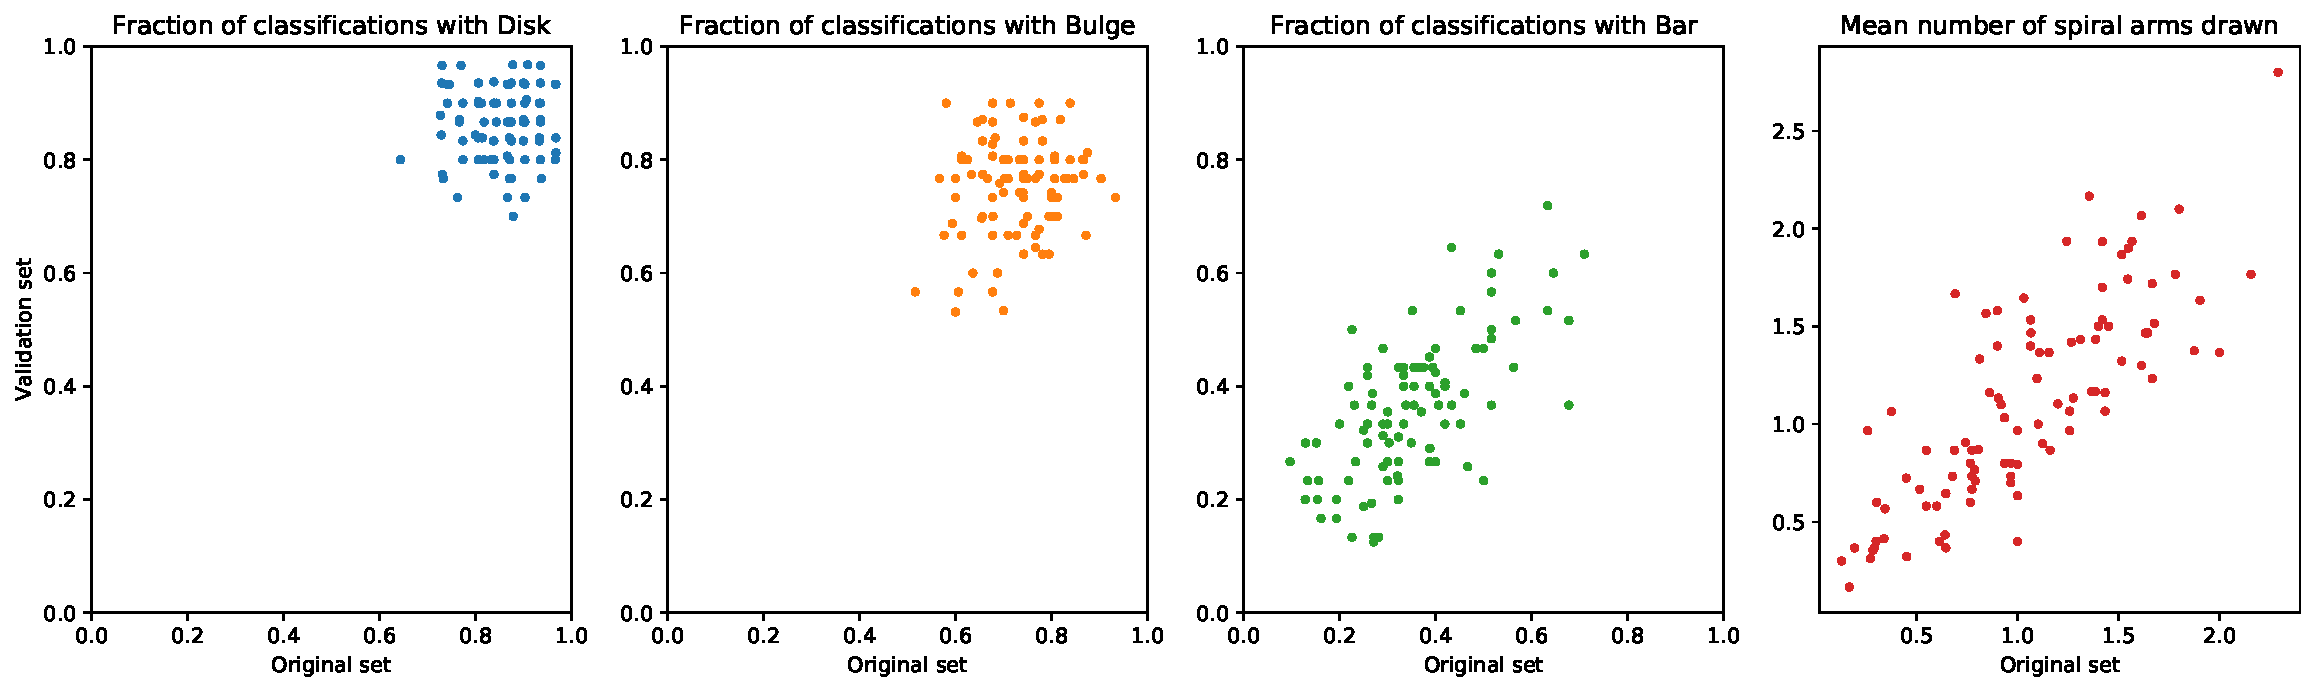
\includegraphics[width=17.3cm]{images__results/component_frequency.pdf}
  \caption{Comparison of frequency of use of component in volunteer models between the original and validation sets of classifications.}
  \label{fig:volunteer_component_consistency}
\end{figure*}

After selecting a component, the volunteer sets its shape and size. We see good consistency in isophotal shape and size, as shown in Figure \ref{fig:aggregate_model_consistency}. The least consistent component is the bar, which may be caused by the lower proportion of volunteers incorporating one into their model. Visual inspection suggests that many volunteers used a very elliptical bulge and drawn spirals to capture the light from the bar. Fewer bars having been drawn by volunteers also has the effect of making clustering more difficult and more uncertain, even for a strongly barred galaxy we effectively go from receiving 30 classifications to around 12 for the bar

\begin{figure*}
  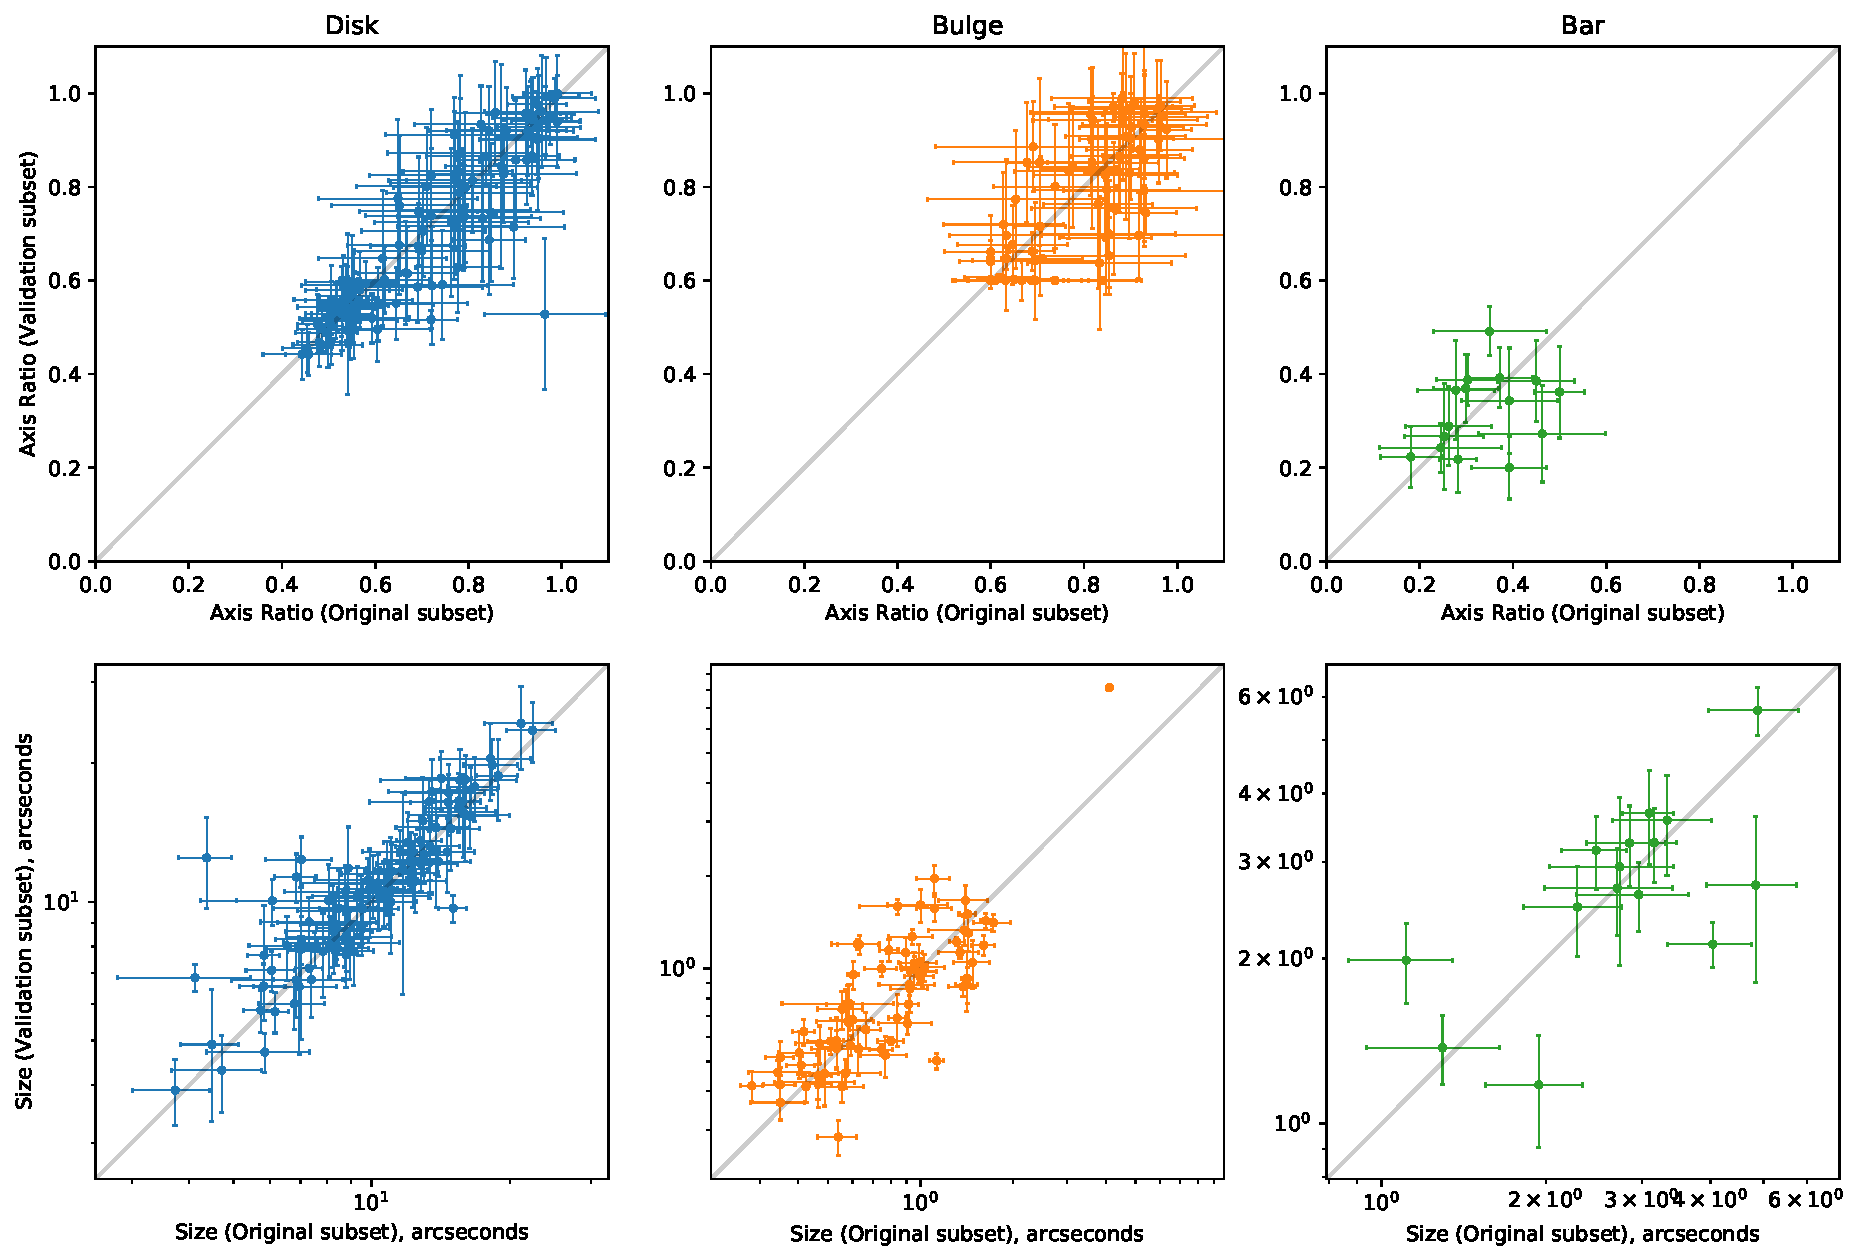
\includegraphics[width=17.3cm]{images__results/component_sizing.pdf}
  \caption{Comparison of component shape in aggregate models between the original and validation sets.}
  \label{fig:aggregate_model_consistency}
\end{figure*}


\subsection{Comparison to results in the literature}

\subsubsection{Aggregated Disk, Bulge and Bar}

After having obtained aggregated models for our galaxies, we examine the reliability of our models through comparison to other results in the literature. For instance, if we compare the axis ratios of the discs recovered from Galaxy Builder to the axis ratio of a 2D S\'ersic fit to the r-band SDSS image of each galaxy (as provided in the NASA-Sloan Atlas), we see excellent agreement (Figure \ref{fig:ax_ratio_comparison}), with an error of $\sim0.1$, consistent with our reported errors. We observe a large number of measurements outside $2\sigma$ around a Galaxy Builder axis ratio of 0.5, which is likely to be due to the drawing tool ellipse having a default axis ratio of $0.5$, and biasing volunteer classification or aggregate shapes.

\begin{figure}
  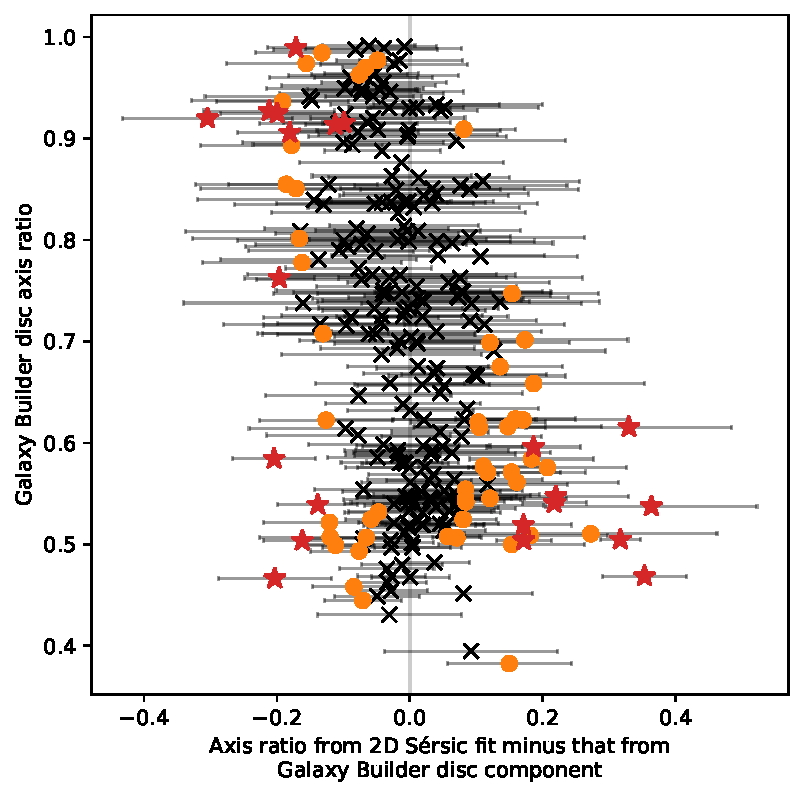
\includegraphics[width=8cm]{images__results/gzb-agg-nsa-comparison.pdf}
  \caption{Difference between the axis ratios of the disc components of aggregated Galaxy Builder models to the results of an r-band S\'ersic profile fit. Points outside 1- and $2\sigma$ are highlighted in orange and red.}
  \label{fig:ax_ratio_comparison}
\end{figure}

We also make comparisons to existing measures of morphology for individual galaxies: When comparing the probability of a classification containing a bar component against a galaxy being classed as strongly-barred or as having no bar (as defined in \citealt{Masters2010:1003.0449v2}), we see a significant difference: classifications of strongly-barred galaxies ($p_\text{bar} > 0.5$) had a \comment{$0.57 \pm 0.16$} chance of containing a bar, vs \comment{$0.37 \pm 0.12$} for galaxies classed as having no bar ($p_\text{bar} < 0.2$). The Spearman correlation between GZ2's $p_\text{bar}$ and the bar likelihood in Galaxy Builder is \comment{$0.75$}, which implies a notable correlation.

\comment{Brooke - Are fits to your galaxies also in Simard et al. (2011), Meert et al, Lackner and Gunn? It would be good to compare to multiple different studies, and since many of them didn’t fit spiral arms or bars it’s a good opportunity to test the effect of adding those components.}


% \begin{figure}
%   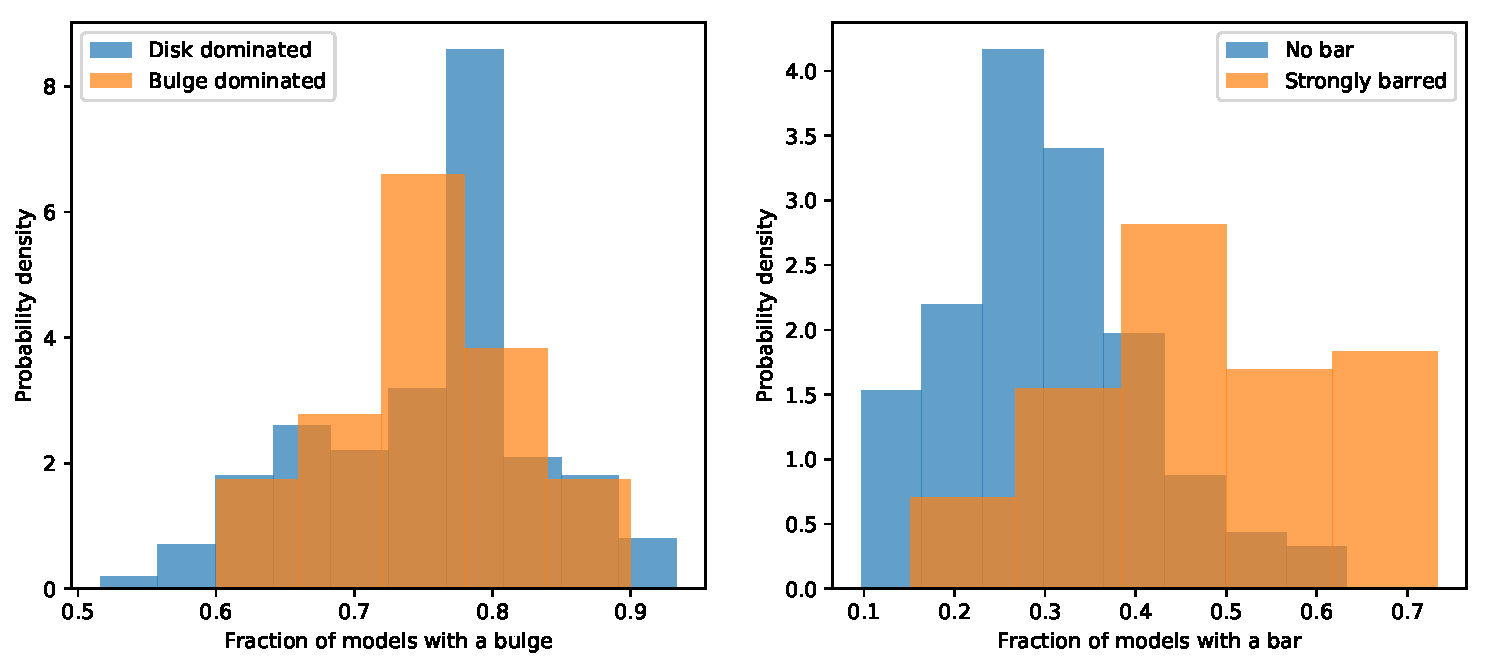
\includegraphics[width=8cm]{images__results/bulge-bar-population-comparison.pdf}
%   \caption{Histograms detailing the differences in model component usage depending on underlying morphology. We see that volunteers consistently use a bulge component regardless of galaxy type (left), but preferentially use a bar for strongly barred galaxies (right).}
%   \label{fig:bulge_bar_comparison}
% \end{figure}

\subsubsection{Aggregated Spiral Arms}
In order to benchmark the reliability of this method of spiral parameter extraction, we compare the result of our logarithmic spiral fit to the relationship obtained by \citet{Hart2016:1607.01019v1} between GZ2 classification and galaxy pitch angle (Figure \ref{fig:hart_pitch_angle}). Their fit was obtained by using the Zooniverse to filter good vs bad spiral arm segments identified using a leading automated spiral arm detection and fitting tool, \textsc{SpArcFiRe} \citep{Davis2014:1402.1910v1}. We find good agreement, although there are large error bars on the GZ2-produced pitch angle (and a caveat in the paper that these pitch angles should not be used for individual galaxies).

\begin{figure}
  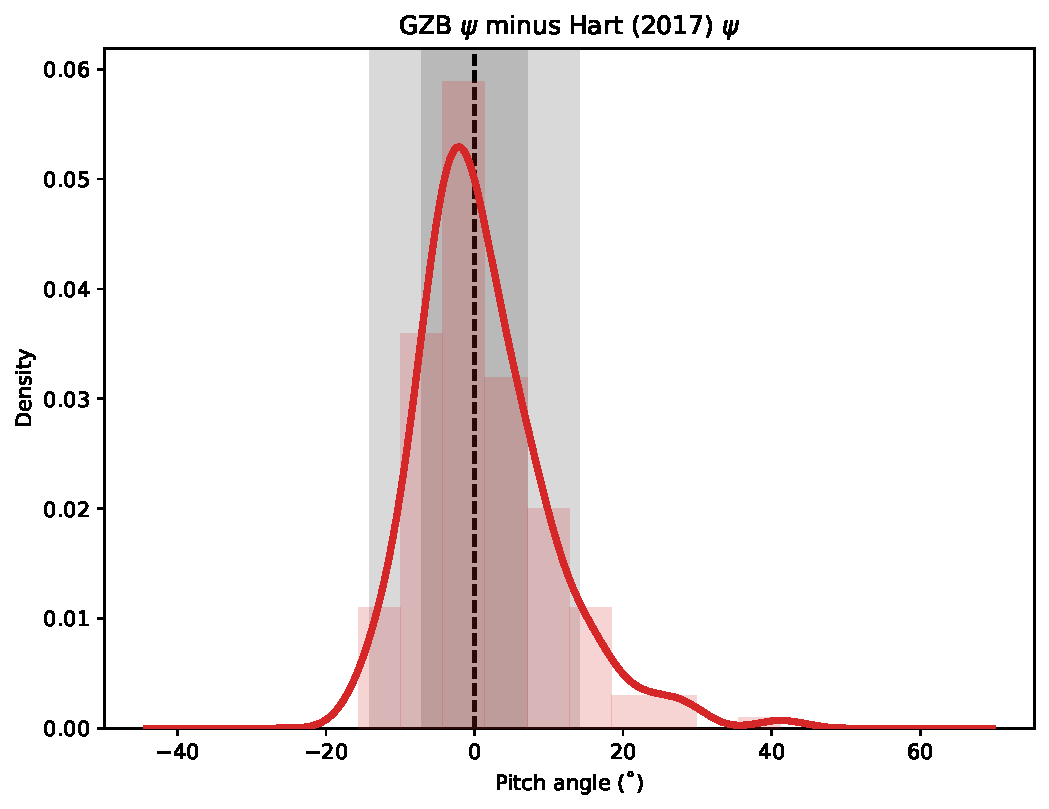
\includegraphics[width=8cm]{images__results/gzb-hart-comparison.pdf}
  \caption{A comparison of Pitch angle obtained by \citet{Hart2016:1607.01019v1} with measured pitch angles for the aggregated model results in galaxies in the Galaxy Zoo Builder sample. The grey regions show 1- and $2\sigma$ errors from \citet{Hart2016:1607.01019v1}. Errors on Galaxy Builder-measured pitch angles are not accounted for.}
  \label{fig:hart_pitch_angle}
\end{figure}

% We can also directly compare the pitch angles from Galaxy Builder models to the output of the SpArcFiRe software, as shown in Figure \ref{fig:sparcfire_pitch_angle}. The SpArcFiRe pitch angle used is the length-weighted mean of all arms of the dominant chirality of a galaxy. In this plot, unlike Figure \ref{fig:hart_pitch_angle}, errors are the sample error of arms used in the averaging and is a measure of inter-arm variation pitch angle.

% \begin{figure}
%   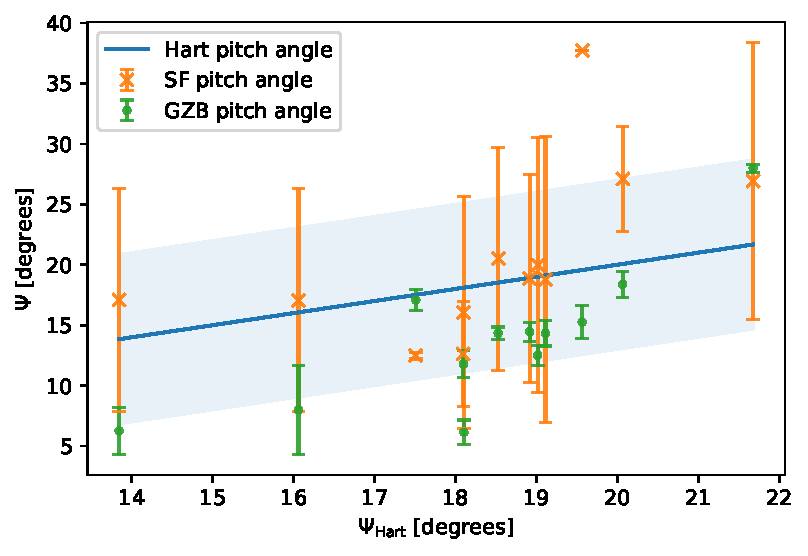
\includegraphics[width=8cm]{images__results/pitch-angle-comparison2.pdf}
%   \caption{A comparison between pitch angles obtained by \citet{Hart2016:1607.01019v1} (blue line) to those obtained through Galaxy Builder and SpArcFiRe. Errors are the sample error of arms used in the averaging and is a measure of inter-arm variation pitch angle.}
%   \label{fig:sparcfire_pitch_angle}
% \end{figure}


\subsubsection{Comparison to Photometric Fits}
In this Section we make comparisons between Galaxy Builder models and the results from other photometric fits in the literature.

One of the largest catalogs of 2D many-component fits is \citet{Simard2011:1107.1518v1}, which performed simultaneous, two-bandpass decompositions of 1,123,718 galaxies in the Legacy area of the SDSS DR7. Three variations of models were fitted: a pure S\'ersic model, an exponential disc and de-Vaucouleurs bulge model, and an exponential disc and a S\'ersic bulge model.

\citet{Kruk2017:1710.00093v2} performed many-component, multi-band decompositions of a selection of Sloan galaxies, 12 of which were also classified in Galaxy Builder. For each of these galaxies we obtain the ``best'' model provided by volunteers (scored using mean squared error, in units of nanomaggies) and futher optimize the slider parameters available to volunteers, as well as the effective radius and axis ratio of all components. Figure \ref{fig:sd_comp_comparison} compares the axis ratios and effective radii of bulges, discs and bars in \citet{Kruk2017:1710.00093v2} to those produced here.

\begin{figure}
  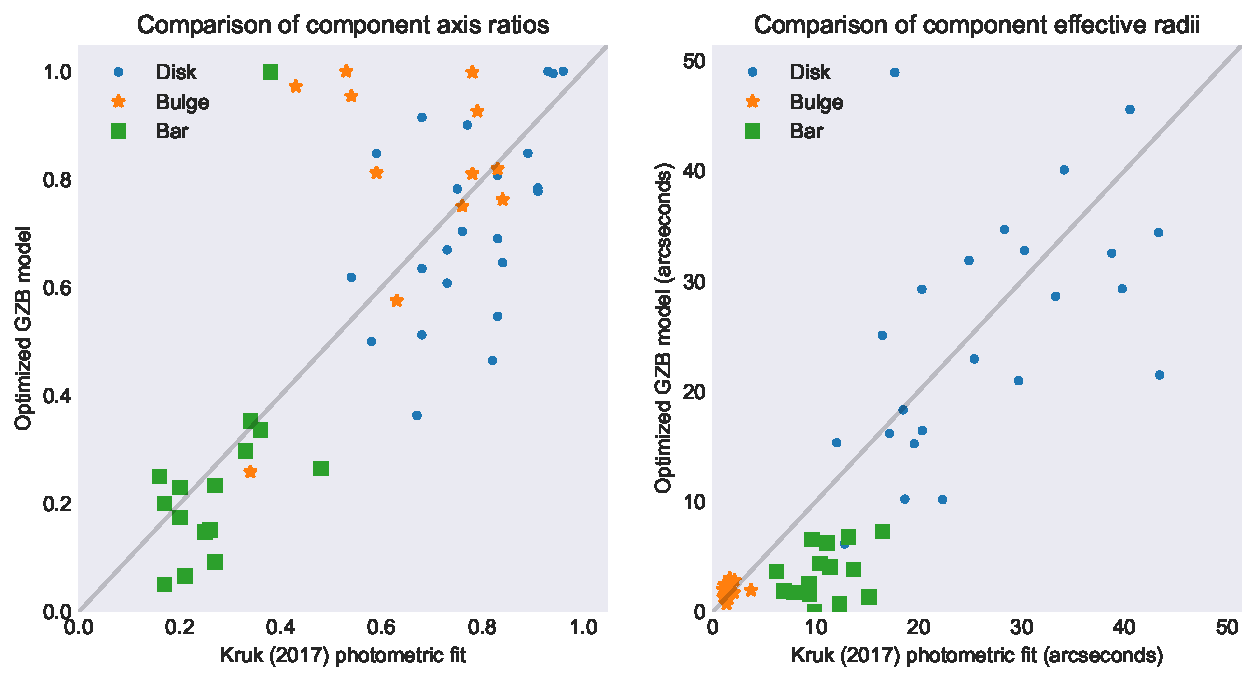
\includegraphics[width=8cm]{images__results/sd_comp_comparison.pdf}
  \caption{Comparison between optimized Galaxy Builder models and the result of 3\-component, multi\-wavelength fits performed by \citet{Kruk2017:1710.00093v2}.}
  \label{fig:sd_comp_comparison}
\end{figure}


\comment{Brooke - I think there's something important missing from this paper: the extent to which using volunteer contributions captures the true set of uncertainties in parametric fitting. Galfit reports formal uncertainties that are very small compared to the true uncertainties. (Chien is the first and loudest person to say this but still people only quote the galfit uncertainties without ever even noting they are only reporting the smallest term.) Studies like Haussler et al. (2007)\footnote{\url{https://ui.adsabs.harvard.edu/abs/2007ApJS..172..615H/abstract}} and Simmons \& Urry (2008)\footnote{\url{https://ui.adsabs.harvard.edu/abs/2008ApJ...683..644S/abstract}} show this in various ways, so this is a known effect that isn’t usually measured for a sample because it’s a ton of work and computing time. GIM2D apparently measures a full set of posteriors, or likelihoods, can’t recall which, but again, it’s not that easy to use that software (by design, because Luc Simard didn’t want it to be a black box) so it’s not as popular as galfit, and there are newer codes like ProFit that do it but they haven’t really taken off yet — and none of these have the advantage of having human eyes on the data. I think this is a unique space and you can potentially make the point that you naturally measure this and thus draw primarily from the advantages of all methods here.

I think this should lean in a little more to the spread in classifiers' fit parameters and explore what that means for a galaxy and whether 30 classifications per galaxy is enough to characterise the uncertainty in the fits
}

\end{document}
